\chapter{TCP/IPの概論}

TCP/IPはいまいちわかりにくいですよね。

インターネットを経由しての通信は、TCP/IPで行われているのは知っているでしょう。でも、アプリケーションから見たとき、TCPとかIPとかがどんな役割をしているから、離れたサーバとクライアントが通信できるのか。また、LANとインターネットとはどんな風に繋がっているのか。そんな部分がよくわからない。

まずは、TCP/IPというもののイメージを掴んでみることにしましょう。

\section{鳥類キャリアによるIP伝送}

伝書鳩でインターネット通信ができる。そのための規格があることをご存知だろうか。

インターネットにおける規格を提案するRFC\footnote{Request for Comment}の1149番で、鳥類キャリアによるIP伝送(IPoAC IP over Avian Carrier)という規格が提案されている。

その名称からなんとなく想像は付くが、これは一体どのような規格なのだろうか。簡単に説明すれば、紙にIPデータグラムの情報を書いて伝書鳩\footnote{規格ではavian carrierであり、伝書『鳩』と明記はされていない}にくくりつけて飛ばす、そうやってデータ通信を行う方法の提案である。\footnote{実際には、鳩の伝送特性、Wormへの対応なども記載されている。}
IPデータグラムという、後に説明する内容に沿った用語を使ったが、要は鳩が運ぶ「情報だと思ってもらえばよい。ここでは、IPデータグラムとは、鳩の脚にくくりつけることのできるサイズの紙に書いた情報である。

このように、IPoACは、鳩に持たせるためのIPデータグラムを作成する規約、鳩の挙動などについて言及し、伝書鳩をインターネットの通信に使用できるようにした規格の提案として提出されたものだ。

種を明かせば、これは毎年4月1日に発行されるジョークRFCと呼ばれるもののひとつである。その中でも、知名度が高く、引用されることも多いのが、このIPoACである。

ジョークRFCではあったが、実証実験は行われている。その実証実験では、パケットロス\footnote{鳩が宛先にたどり着かなかった状態を指す}が多く、伝送遅延も大きい。つまり、ものすごく時間がかかるという、ある意味当然の結論が出た。だが、伝送遅延を許容し、たくさんの鳩を用意できるなら、伝書鳩でインターネットの通信を行うことは可能である。実用的ではないが、TCP/IPは、伝書鳩でも通信を行うことが可能なプロトコルである。それについて説明していこう。



\section*{}
\begin{itembox}[l]{いもうとコラム 惑星間インターネット}
RFC1149はいわゆるジョークRFCでしたが、、インターネット通信において、情報伝達に鳩を使う以上に、送ったデータのロストや応答時間(レイテンシ)が大きくなる環境があります。

それは、宇宙です。さよならジュピターでも、探査船のコンピュータと月に設置されたコンピュータがレイテンシを越えて会話するシーンがありましたね。\footnote{スペースアロー搭載のナヴァホと月のティム・ラビット}

このような環境のインターネット通信は、惑星間インターネット(Interplanetary Internet)として研究開発が行われています。
\end{itembox}


\section{伝書鳩でインターネット通信ができるのはなぜか}
鳩は遅い。そして、送り出した鳩が必ず通信相手にたどり着くわけでもない。また、順番通りに届くわけでもない。だが、鳩を伝送媒体に用いて、でインターネットで行われている通信が成立する。それはなぜなのだろうか。

その答えとは、伝送遅延を許容し、鳩は確率的にしか相手のところにたどり着かず、送り出した順番と到着した順番が一致しないことを前提に通信の仕組みを作ればよい。つまり、鳩に完璧さを求めなズ、それをサポートする側でなんとかするわけだ。では、鳩が果たす役割について考えてみることにしよう。

伝書鳩の役割とは、通信を行う双方の間で、IPデータグラム、つまり情報を物理的な空間を越えて運ぶことである。そして、鳩の役目とはそれだけである。後ほど説明する言葉を使えば、物理層とネットワークアクセス層に相当する。

鳩なので、途中で餌になる虫を見つけたり、交尾相手を見つけてふらふらとそちらに飛んでいくことがある。鷹に追いかけられて逃げたりするかもしれない。そして、そんな鳩は到着が遅れたり、場合によっては相手のところに到着しないこともある。もちろん、送り出した順番に鳩が到着するわけでもない。多分、順番はぐちゃぐちゃだろう。

実際、これらのことはIPoACの提案にもあり得る事態として記載されている。

まず、鳩が相手のところにたどり着くことを期待することにしても、鳩なのだから、必ずしも相手側に到着するわけではない。これは重要な前提であるので、忘れないでいてほしい。。



\subsection{鳩で通信するための前提条件}

この、IPoACによる通信にみっつの前提条件を追加する。

前提条件の一つ目として、鳩が届けたIPデータグラムを受け取った側は、それが判別可能であれば、鳩を使って「読めるデータを受け取った」という返事をしなければならない。つまり、鳩が到着し、その運んできたデータが利用可能なものであれば、鳩に「読めるデータを受け取った」という情報を持たせて相手に向けて飛ばすわけだ。

ここで、電話を使って鳩の到着を連絡すればよいと思うかもしれない。だが、電話を使える状況なら、最初から電話で通信して、鳩を使って通信しなくていいではないか。

前提条件の二つ目は、送信側は、一定時間待っても「到着した」ことを知らせる鳩が来なければ、先に送り出した鳩と同じIPデータグラムを持たせた、新しい鳩を送り出さなければならない。

これは、相手が「読めるデータを受け取った」ということが確認できるまで3は、そのデータは届いていないと見なすということである。

三つ目は、データには、送信した順番を再現するための通し番号を書いておくということである。「受信した」メッセージには、その番号も書き添え、何番目のデータを受け取ったかがわかるようにする。

では、そのルールのもとで、伝書鳩を使って通信する手順を定義していこう。メッセージを送り出し、相手が受信したのを確認する手順を列挙しよう。

	\begin{enumerate}
		\item 発信側がメッセージを作成する
		\item メッセージに番号を付ける
		\item 発信側が鳩を飛ばす
		\item 受信側に鳩が到着したら、持ってきたデータを確認する
		\item 受信側でデータが正しいことを確認できたら「到着した」という情報を持たせた鳩を発信側に飛ばす
		\item 発信側に「到着した」の情報をもった鳩が到着したら、発信側は自分が送り出した鳩が無事に到着したと判断する。
		\item 発信側は,一定時間内に「到着した」ことを知らせる鳩がこなければ、それに対応する情報についてはもう一度別の鳩に持たせて送り出す。これを、「受信した」メッセージを受け取るまで繰り返す。
	\end{enumerate}

この手順を用いると、送信側、受信側のどちらかが飛ばした鳩が無事に到着しなくても、鳩を送り直すことを繰り返せば、最終的に通信は成立する。鳩がたくさん必要なのは、何度同じ情報を持たせた鳩を飛ばすことになるか、事前にわからないためだ。

\subsection{鳩の宛先をどうあらわすのか}
次に、鳩がどこに向かって飛ぶのかを考えてみよう。伝書鳩は、ある宛先にむけて飛ぶように訓練される。もう一度書くならば、宛先ことに、そこに向けて飛ぶ鳩がいて、宛先を決定したら、どのは都を使うかが決まる。

では、人間はその宛先をどのように管理するのだろうか。ここでは、住所を使うことにしよう。そうすることで、鳩を管理する人間が、どこに飛ぶ鳩を使うのか管理しやすくなる。

突然だが、京都市は、住所の表し方が二つある。ある場所を表すのに、通常の何区何町何丁目何番地、という表し方がひとつ。街路が碁盤の目になっている京都では、場所のブロックがどの通りに面しているかを、東西方向、南北方向の通りの交差点から、東西南北どちらに進めばいいかで表現していた。

例えば、京都市役所は、現在使用されている住所表記では京都市中京区押小路河原町西入榎木町450-2であるが、古い表記では京都市中京区寺町通り御池上ル本能寺前である。そして、京都市役所を宛先とする郵便を出せば、このどちらで記載しても届く。\footnote{京都では、古い住所表記に使われる通りの名前を、「まるたけえびすに、おしおいけ、あねさんろっかく」というような歌にして覚えていた。この歌はいくつかあるので、興味があれば調べてみてほしい。}

京都の住所表記の話を持ち出したのは、鳩が飛んでいく先である、ひとつの場所を表すのに複数の表現方法があるためだ。古い表記は比較的おおざっぱ、新しい表記は細かい。だが、実際の地図上の場所は同じである。

新しい表記は、より細かく場所を特定することができる。つまり、本能寺前に市役所以外の建物があったとしても、市役所とは別の住所で表すことができるだろう。

だが、そんな違いがあったとして、メッセージを作る人間は、「京都市役所」にメッセージを送ってという指示だけ出せばいい。住所の表記の違いは、はとを飛ばす担当者が、京都市中京区寺町通り御池上ル本能寺前「」に向けて飛ぶ鳩を使うのか、京都市中京区押小路河原町西入榎木町450-2「」にむけて飛ぶ鳩を使うのか、使い分けを意識すればいい。

この二つの表記が、後に説明するIPv4とIPv6に相当する。つまり、鳩を洗濯するやり方は二つある。

\subsection{発信側と受信側の協調}
次に、IPoACで、発信側と受信側はどのくらい協調して通信を行うか、それについて見直してみよう。ここでいう協調とは、お互いにタイミングを申し合わせて動くことであるとする。

前提として、この両者は、鳩以外の情報伝達手段を持っていない。変な言い方ではあるが、我々はインターネットで通信を行う際に、インターネットしか情報伝達手段を持っていない。\footnote{特に、トランスポート層について学習する際に、それを思い出してほしい。}

発信側は、IPデータグラムを送る必要がある場合は、受信側への事前連絡なしに鳩を放つ。ここでは鳩より早い情報伝達手段がない。そのため、事前連絡のしようもない。

一方の受信側は、いつ鳩がきてもいいように受け入れる準備はしている。だが、鳩がこない限りは何もしない。鳩より速い通信手段はないのだ。もとより送信側に連絡を取りようがない。

受信側から送られる「到着した」情報についても同様である。受信側は、送信側への事前連絡なしに「到着した」という返事を持たせた鳩を放つ。発信側は、「到着した」の鳩がいつ来てもいいように準備はしている。だが、鳩が来ずにに時間切れになったら、こんどは送信側が受信側への事前連絡なしに、先ほど送り出した鳩と同じIPデータグラムを持った鳩を送り出す。

このやり方は、TCP/IPにおけるTCPと呼ばれつ通信手順に相当する。

\subsection{鳩の順番が違っていた場合}
到着した鳩の順番が違うことは、当然あり得ることだ。たとえば、1番データを持った鳩が来たが、次に来たのは3番のデータを持った鳩であったとする。2番のデータが来てないことはどう連絡すればいいだろうか。

受信側の行動の正解は、2番のデータに関しては何もしないことである。2番が「受信できた」というメッセージが来なければ、送信がわは2番のデータを別の鳩に着けて送り出さなければならない。それによって、時間はかかるが順番も含めての確実な通信が可能となる。


\subsection{受信を知らせるのが面倒くさいときの通信}
ここまで説明した方法は、「受信した」メッセージのやり都市が成立するまで、データの再送、つまり鳩が再び放たれ続ける。正直なところ、これは面倒だし、順番の雁も含めて考えると、送信側、受信側ともにコストが高い。なので、「受信した」確認を市内通信というものがある。

たとえば、一匹の鳩の脚にくくれる程度の問い合わせと、おなじく一匹の鳩の脚にくくれる答えで終了する通信があるとする。このとき、「到着した」という連絡にかける手間は、行われる通信に対してあまりにも大きい。そのため、確実性がなくてもかまわない場合は、「到着した」連絡を省略することで、通信のコストダウンを計ることができる。

このような、受信を確認せずに送ってしまうやり方が、TCP/IPにおけるUDPに沿うとする。

\subsection{鳩と人間の役割分担}
次に、IPoACを使った通信での、鳩と人間の役割分担について考えてみよう。そのために、鳩と人間がIPoACにおいてどのように振る舞うかを再確認したい。

\subsubsection{鳩の性質}
IPoACによる通信では、鳩は、「IPデータグラムを運ぶ」のが役割である。それ以外の役目は持っていない。発信側から受信側に飛ぶだけである。そして、送り出した順番で到着する保証もない。繰り返すが、鳩は、受信側にたどり着く義務すら負っていない。

これは伝書鳩の性質でもあるのだが、鳩は決められた宛先、つまり」巣に向かって飛ぶ。違う宛先に鳩を届けるなら、そこに向かって飛ぶ鳩にデータを持たせるわけだ。

鳩が運ぶIPデータグラムがたどり着いたか、たどり着いていないかを判断し、たどり着いていないと思われる場合に別の鳩を送り出すのは、鳩を飛ばす人間の役目である。

伝書鳩は、決められた先に帰巣本能に従って飛ぶ。大事なことなのでもういちど書くが、宛先毎に、そこに向けて飛ぶ鳩がいると考えてほしい。

\subsubsection{人間の役割}			

次に、通信に関わる人間を増やして、その担当する仕事を分解していく「。

まず、メッセージを送りたい人の依頼でメッセージを作成する人物がいる。

次に、その人からメッセージを預かり、データとして次の担当に渡す役割の人物がいる。この人物が、実は一番仕事が多い。

この人物は、「受け取った」メッセージが届いたかのチェックも担当し、届いていないときは、同じデータを再度送り出す役割もある。
また、鳩が持ってきたデータの順番を確認する役目も持っている。データの順番がおかしければ」受信した」メッセージを送らないことで送信側にそれを伝える。

その次に出てくるのは、前の担当者から預かったデータの宛先を見て、どこ宛ての鳩に着ければいいかを判断する。また、この担当者は、鳩が来たらそれを受け入れ、データを前述の担当者に渡す。この担当者が気にするのはどこ宛ての鳩を飛ばすかであって、鳩が持ってきたデータについては何も気にすることはない。




\section{IPoACとインターネットプロトコルモデル}
では、実際のインターネットにおいて、鳩はどこにいるのだろうか。正確に言えば、鳩に相当するのはどの部分なのだろうか。それを考えるために、IPoAC二関わる人間と鳩を、役割毎に層にしてみよう。
\begin{table}[hbtp] 			
\begin{center} \label{hatostack}
	\begin{tabular}{l}  \toprule
		役割 \\ \midrule
		メッセージをデータとしてを作る \\
		データの送信を管理し、対応する「到着した」の到着をチェックする \\
		宛先毎に鳩を選び、送り出し受け入れる \\
		パケットを運ぶ \\ \bottomrule
	\end{tabular}
\end{center} \caption{人と鳩の役割分担}
\end{table}

役割ごとに上下に重ねて書くと、表\ref{hatostack}となる。この表では、ある役割の者は、表で直上に書かれた者から依頼を受け、直下の役割の者に作業を任せる。どういうことかというと、鳩は必ず、鳩の受け入れ担当者にのみIPデータグラムを渡す。到着とその返事を管理している者に対してはなにもしない。逆に、到着と返事を管理する者が、直接に鳩を送り出すこともない。

そして、鳩を送り出し受け入れる担当者は、鳩が持ってきたIPデータグラムを、到着と応答を管理している者に渡す。また、「到着した」返事を送る指示を受けたら、それを鳩に持たせて送り出す。

つまり、各担当者、そして鳩は、表\ref{hatostack}で、直接上下に接している相手からのみ指示を受け、指示をする。これをインターネットの用語に置き換えてみよう。説明はこの先で行うので、今はインターネットでの用語が何になるかだけ見てもらうのでかまわない。

\begin{table}[hbtp] 
\begin{center} \label{hatostack2}
	\begin{tabular}{ll} \toprule
		役割 & インターネットでの名称 \\ \midrule
		メッセージをデータとしてを作る & アプリケーション層 \\
		データの送信を管理し、対応する「到着した」の到着をチェックする & トランスポート層 \\
		鳩を選び、送り出し受け入れる & インターネットプロトコル層 \\
		パケットを運ぶ & ネットワークアクセス層 \\ \bottomrule
	\end{tabular}
\end{center} \caption{インターネットの用語との対応関係}
\end{table} 

このように、メッセージを作るものをアプリケーション層、データの創出を管理し、必要なら再送するのがトランスポート層、あて先を見て鳩を選ぶのがインターネットプロトコル層、鳩がネットワークアクセス層とよばれるそれぞれの層(レイヤー)に相当する。

この四つの機能が菱餅のように重なり合っているイメージでとらえられることから、いわyるるTCP/IPのことを、インターネットプロトコルモデルと呼ぶ。


\section*{}
\begin{itembox}[l]{いもうとコラム IPoACは何を定義しているのか}
実際のところ、IPoACは何を定義しているのでしょうか。それをインターネットプロトコルスイートの言葉を使うと、ネットワークプロトコル層である鳩に、どのようにインターネットプロトコル層でのデータを載せ、取り扱うのか、という部分になります。

これは名前からもわかることで、IPデータグラムを鳩に乗せて運ぶから、IP over Avian Carriersとなるのです。

\end{itembox}


\section{インターネットプロトコルスイートとTCP/IP}

\begin{table}[hbtp] 
\begin{center} \label{internetprotocolsuite}
	\begin{tabular}{l}  \toprule 
		レイヤ名 \\ \midrule
		アプリケーション層 \\
		トランスポート層 \\
		インターネットプロトコル層 \\
		ネットワークアクセス層 \\ \bottomrule
	\end{tabular} \caption{インターネットプロトコルスイート}
\end{center}
\end{table}

インターネットの通信方法であるTCP/IPは、このように、役割分担したいくつかの機能を組み合わせることでできている。なので、このモデルをインターネットプロトコルスイート、と呼んでいる。また、その機能の一つ一つに層(レイヤ)という言葉がつくのは、表\ref{internetprotocolsuite}のように、上下に層となって重なっているように表されるためだ。


では、ここまで何となく使ってきたTCP/IPという用語は何であろうか。TCPはトランスポート層のプロトコルの一つ、IPはインターネットプロトコル層のプロトコルの名称である。一見すると、表\ref{internetprotocolsuite}の、トランスポート層とインターネットプロトコル層のプロトコルの名前をつなげただけに見える。

だが、この名称で、四層からなるインターネットプロトコルスイートそのものをあらわしている。そのため、単にTCP/IPと言うときは、インターネットプロトコルスイートであると考えてよい。

\subsection{レイヤの上下関係とサービス}

\begin{wrapfigure}[17]{r}{6cm}
	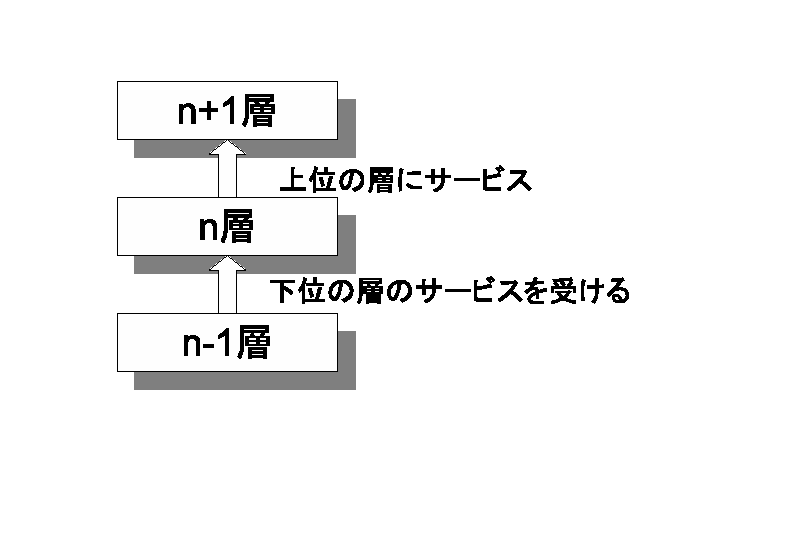
\includegraphics[width=6cm, clip]{draw/service.eps}
	\caption{レイヤの上下関係}
	\label{fig:service}
\end{wrapfigure}

ここまでの説明の表現を変えて書き直せば、インターネットプロトコルスイートの各層は、自分より下の層が自分にサービスすることを前提に、自分より上の層に対してサービスを行う。

もういちどIPoACで説明すれば、インターネットプロトコル層の担当者は、ネットワークアクセス層である鳩から「IPデータグラムを運ぶ」というサービスを受ける。そして、インターネットプロトコル層の担当者がトランスポート層である、上位の担当者に対して、提供するサービスは、回されてきたメッセージをどの鳩に載せて運ぶかを選択し、送り出すという仕事である。

このように、下位の層からサービスを受け、上位の層に対してサービスを行うことを、$n$層のサービスは、$n-1$層からサービスを受け、$n+1$層にサービスする、といううように言い表す。

\subsection{レイヤ間の依存関係}

次に、層と層の間の依存関係について考えてみよう。実は、それぞれの層は、お互いに全く依存しあわない。鳩を使うかわりに、糸電話を使っても、瓶詰めの手紙を海に流しても、はじめてのお使いをする姪っ子に持たせても、通信は成立する。\footnote{このことを表す言葉として、Two can and tin. というフレーズがある。意訳すれば「糸電話でもいいよ」となる。}

これは、あるレイヤは、直接に接していないレイヤのことは全く気にする必要がないと言うことでもある。トランスポート層の担当者は、情報のやりとりに使われているのが鳩なのか糸電話なのか、それとも姪っ子なのかを考える必要がない。

また、本書ではインターネットプロトコル層について、バージョン4のいわゆるIPv4とバージョン6のIPv6の両方について、説明を行う。インターネットプロトコル層は、IPv4でもIPv6でも、トランスポート層、ネットワークアクセス層は、プロトコルの変更なく通信を行うことができる。\footnote{実装の観点で見れば、インタフェイスの違いなどから、全く変更が必要ないわけではない。}

トランスポート層の置き換えの例もある。インターネットの通信でWAN高速化を行う機器がある。これは、対抗する機器の間でトランスポート層で、TCPやUDPなどの従来のプロトコルと違うものに置き換えて、通信時間の短縮を計る。

では、トランスポート層を置き換えても、通常のインターネットを経路として通信できるのはなぜだろうか。途中の経路はインターネットプロトコル層のプロトコルで通信が行われる。そのため、トランスポート層になにを使っても、インターネットプロトコル層から見れば、同じIPデータグラムの運ぶデータとなる。そのため、インターネットプロトコル層では何の変更もなく通信が可能である。

\subsection{プロトコルスタック}
ここまで説明したように、TCP/IPは異なった役割をもつプロトコルが、お互いにサービスを提供したりされたりして成り立っている。図にすると、各層のプロトコルを上下に重ねたように表される。このように、役割を分けたプロトコルが上下に重なる形で全体像が作られるプロトコルスイートを、プロトコルスタックと呼ぶことがある。

プロトコルスタックという呼び方は、TCP/IPなどのプロトコル実装の場面で使用されることも多い呼び方である。例えば、プロトコルスタックを実装すする、という言い方をする。

\section{エンドツーエンド原則}
TCP/IPには、二つの意味を持つエンドツーエンド原則というルールがある。では、二つある意味とは何であろうか。

\subsection{処理は両端(エンド)でのみ行い、途中の経路は導管に徹する}

一つ目は、アプリケーション層やトランスポート層による制御は通信の端点、つまりエンド側でのみ行い、途中の経路は通信の導管に徹するべきである、ということである。TCP/IPの用語で言えば、途中の経路はインターネットプロトコル層の通信をさす。そして、トランスポート層やアプリケーション層での通信が途中に介在しない。

この原則があるので、先ほど説明したように、通信のエンドでWAN高速化機器を使用したとしても、通常のインターネットで通信を行うことが可能となるわけだ。

このように、途中経路の実装を簡単にして、経路の敷設を行いやすくしていたのだ。\footnote{昔はトランスポート層以上の実装には、かなりのリソースを必要とした。そのため、重い処理をするノードを減らしたいという意味もあった。}

\subsection{通信の両端は常に対等である}

もう一つは、インターネットに接続されたすべてのエンドは、対等な立場で通信が可能であるべきという原則である。対等な立場というのは、インターネットに接続されたすべてのホストは、自分を含むすべてのホストに対して送信を行うことができ、逆に、すべてのホストからの通信を受信できるべき、ということである。

もっとも、現在のインターネットはこのエンドツーエンド原則の理念が、多くの場合において失われている。OBP25と呼ばれる、あるインターネットプロバイダに接続されたホストからは、そのインターネットプロバイダが外にあるメールサーバに直接接続できない様にする制限などは、一つ目の原則に反する者であると言えよう。

また、IPv4のアドレス不足の対策として現在家庭や企業で多く使用されるNAT\footnote{Network Address Transrate 一つのグローバルなIPアドレスを複数のホストで共用するための技術の一つ。NAPTやIPマスカレイドなど、いくつか呼び方がある}は、後者の原則に反している。

もっとも、エンドツーエンド原則が提唱された当時は、インターネットに接続していた組織がすべて顔見知りであった、いわゆる性善説が成り立っていた時代であることを記載しておかなければ不公平になるであろう。残念ながら現在は、エンドツーエンド原則を崩さねばならないこともある時代である。

\section*{}
\begin{itembox}[l]{いもうとコラム 実際のエンドツーエンド}
エンドツーエンドは、今ではあまり現実的でない考えであるという見方もあります。たとえば、プロキシやファイアウオールは、インターネットプロトコル層よりも上のレイヤーで通信を処理し、中継したり、通信を断ったりします。

それでも、両端から見てインターネット層の通信で結ばれているように見えれば、通信は成立するということでもあります。それが、インターネットプロトコルの通信を、アプリケーション層のデータとして運ぶ「トンネル」の考え方につながっています。


\end{itembox}


\section{レイヤごとの役目}
では、各層の役目を、もう少しだけ、インターネットの用語を使って説明し直そう。

\subsection{ネットワークアクセス層}
同じネットワークの中で、ネットワークに接続されたインタフェイスを区別し、通信するための層である。「同じネットワーク」とは、二つ以上の機器が、共有する伝送媒体によって直接に接続されたものであるとする。もう一度書くと、IPoACにおける鳩は、ネットワークアクセス層である。

ケーブルや信号などの電気的な規格と、それを利用してでどのような情報を送るか、それらをまとめが概念がネットワークアクセス層である。

概念、と書いたのは、ネットワークアクセス層そのものはTCP/IPでは定義されていない。本書では後の章で、説明のためにPPPやイーサネットを取り上げているが、これらはインターネットプロトコルスイートの中で規格されたものではない。


\subsection{インターネットプロトコル層}
インターネットプロトコル層は、ネットワークアクセス層でいうネットワークが複数あった場合に、そのネットワークとネットワークの間での通信を担当する。ただし、インターネットプロトコル層は、ネットワーク間の通信手段を提供するのが役目であり、エンドツーエンドで通信が成立しているかは保証しない。

TCP/IP関連の用語で最もよく名前を聞くであろうIPアドレスは、インターネットプロトコル層でネットワークとそこに接続されたホストを特定するための識別手段であり、インターネットにおける文字通りの住所である。

インターネットプロトコル層では、これまで使われてきたIPバージョン4と、より多くのIPアドレスが使える、新しい規格のIPバージョン6という、二つのバージョンのインターネットプロトコル層の規格が、2016年現在は併用されている。このように併用されていることを、インターネットプロトコル層が二つある、という意味で、デュアルスタックと呼ぶ。

\subsection{トランスポート層}
トランスポート層には大きく二つの役割がある。一つは、ポート番号とよばれる、通信を行うアプリケーションを特定するための番号を提供して、一つのIPアドレスを用いて複数のアプリケーションが同時に通信できるようにする、多重化である。

もう一つは、エンドツーエンドでの確実な通信を担当することである。確実な通信が成立している条件は、通信相手がデータを受信したことを確認した状態であるとする。また、データの到着順、つまり通信内容の送信順を確認して、受信側でその順番を再現する、つまり、通信の順番も担保している。

この役割を持つのが、トランスポート層のTCPである。


また、IPアドレスの多重化だけを行うプロトコルもあり、こちらがUDPとなる。

TCPとUDPは、アプリケーション層の通信の性質によって、使い分けられる。


\subsubsection{コネクションとコネクションレス}
TCPのように、確実な通信を行うプロトコルは、その動作から通信のエンド同士が直接接続されているかのような状態をエミュレートしていると言うことができる。そのため、コネクション型、もしくはコネクション指向の通信と呼ぶ。

一方のUDPは、確実な通信を行うために必要な、「受信した」追う乙の送出やデータの到着順の管理などは行わない。つまり、コネクション指向の動作はおこなわない。そのため コネクションレス型と呼ぶ。


\subsection{アプリケーション層}
アプリケーション層は、通信のエンドとエンドで通信を行う主体である。つまり、TCP/IPというのは、このアプリケーション間の通信を行うために存在すると言っていい。

アプリケーション層とは、トランスポート層以下が提供する通信を使って、他のプロセスと通信するプロセス、つまり、アプリケーションである。たとえば、メールサーバやメールのクライアントソフトは、アプリケーション層となる。

他のホストの別のアプリケーションと通信するときの規約は、アプリケーション層のプロトコルと呼ばれる。また、アプリケーション層のプロトコルごとに、トランスポート層でTCPを使うか、UDPを使うかが決められる。

たとえば、SMTPやHTTPといった、確実な通信を前提としたプロトコルを使用するときは、トランスポート層にTCPを使用する。また、DNSのような、応答に対して「受信した」通信のコストが高いプロトコルや、SNMPのようにひたすらデータを待つプロトコルの場合は、UDPが使用される。



\section{カプセル化トンネリング}

実際にインターネットプロトコルスイートで通信を行う場合は、カプセル化とトンネリング、という二つの概念を意識することとなる。それについて説明を行おう。

\subsection{カプセル化}

\begin{figure}
	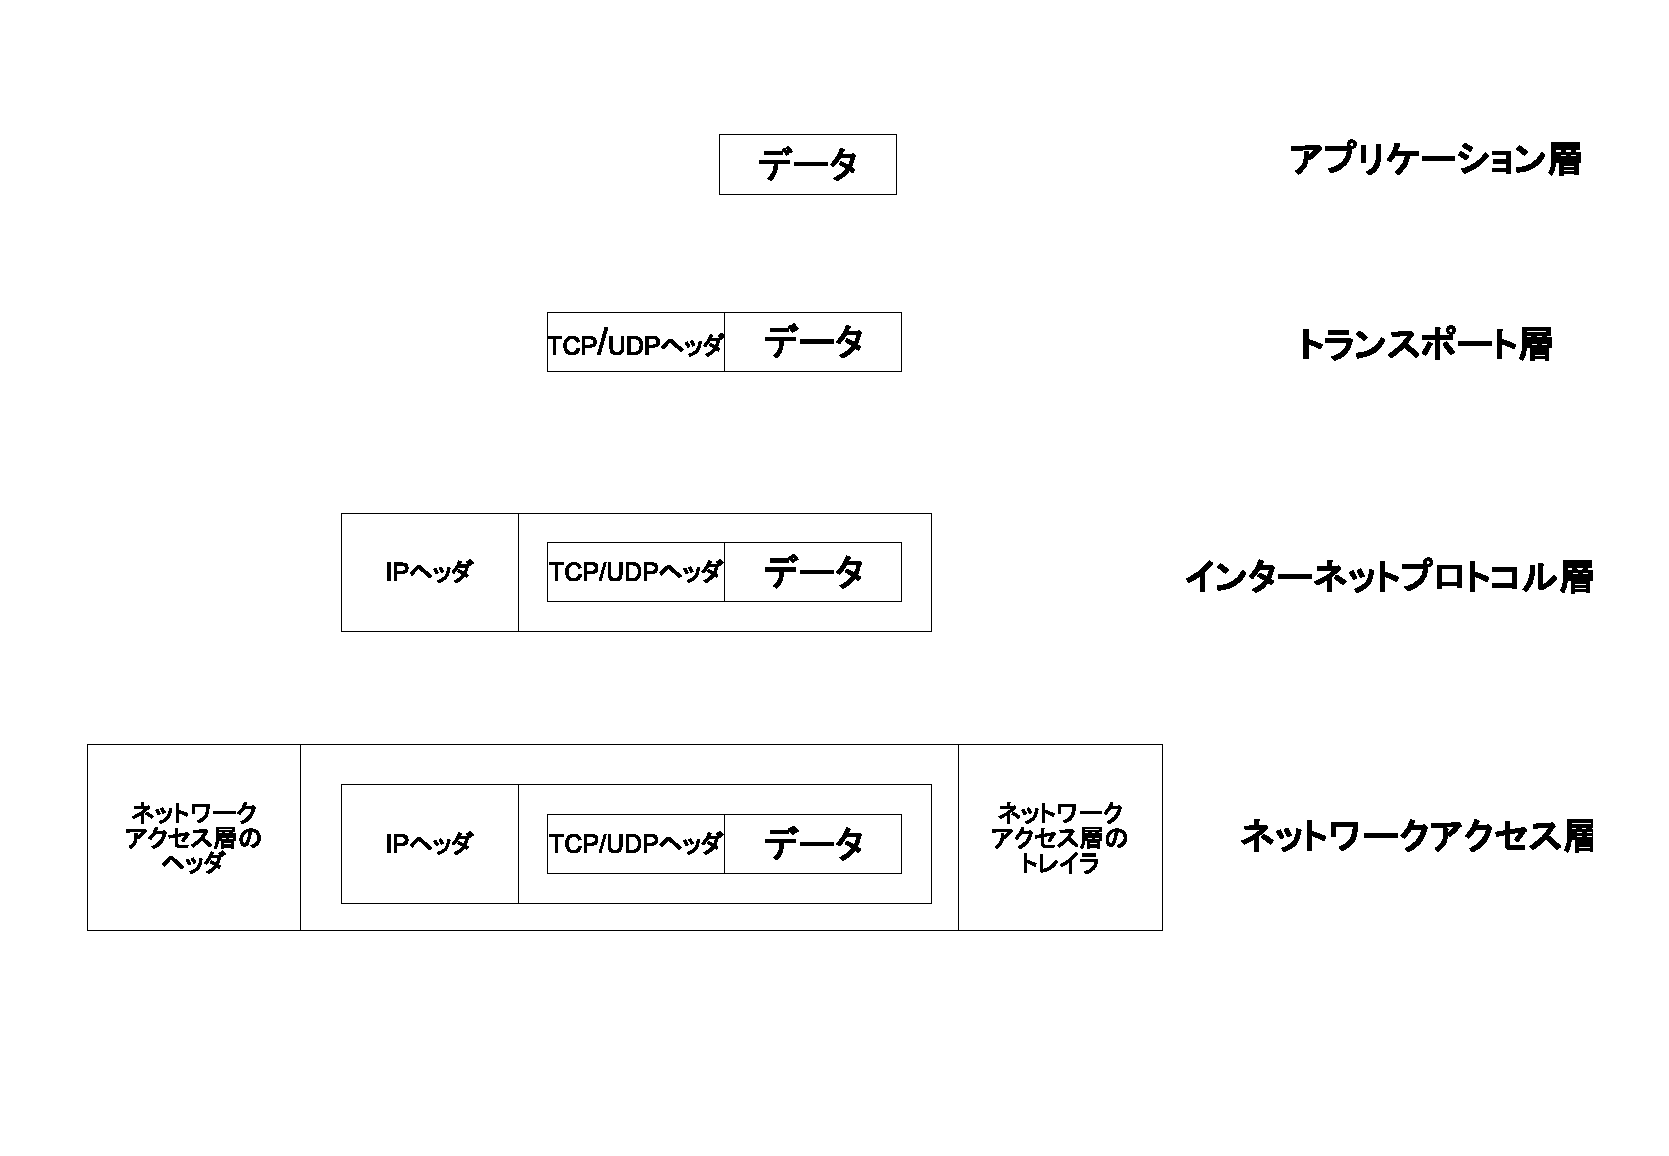
\includegraphics[width=12cm,clip]{draw/encupselation.eps}
	\caption{カプセル化}
	\label{fig:encupselation}
\end{figure}

TCP/IPのように、複数のレイヤからなるプロトコルには、カプセル化という概念がある。

今度は、実際のデータの流れを考えてみよう。アプリケーション層から発行されたデータは、トランスポート層で扱えるデータにしてやらないと、トランスポート層から送り出すことができない。
トランスポート層から送り出せるデータにするには、トランスポート層のデータとして必要なデータを追加する。このデータの追加を、カプセル化と呼ぶ。粉薬をカプセルに入れて形を変えるイメージでそう呼ばれるのだ。

このカプセル化は、アプリケーション層のデータをトランスポート層に送り出すときだけではない。トランスポート層から送り出されたデータは、インターネットプロトコル層で扱えるようにする必要がある。このときも、インターネットプロトコル層に必要なデータを付加する、カプセル化が行われる。

更に、インターネットプロトコル層からネットワークアクセス層にデータが送り出される際も、同様にカプセル化が行われる。

最終的に、アプリケーション層のデータは、トランスポート層、インターネットプロトコル層、ネットワークアクセス層という三重のカプセルに包まれて送り出されるされる。

\subsection{カプセルをはがす}
では、受信側に届いたデータはどうなるのであろうか。データを受信したネットワークアクセス層は、ネットワークアクセス層で通信するためのデータを外し、インターネットプロトコル層にデータを渡す。インターネットプロトコル層、トランスポート層でも同様に、自分が通信に使うデータを外して、一つ上のレイヤに残りデータを渡す。

最終的に、アプリケーション層は、送信元のアプリケーション層が発信したデータのみ受け取る。

\subsection{トンネリング}
トンネリングという言葉には、二つに似て異なる意味がある。

インターネットプロトコルスイートのあるレイヤとレイヤの間の通信は、いわば同じ階層にあるレイヤの間でトンネルを通しているようなものである。そのため、同じ階層にあるあるレイヤからレイヤへの通信を、トンネリングという。

トンネリングは、カプセル化を、通信のエンドから見た視点で説明したものである。

だが、トンネリングにはもう一つの側面がある。同じ階層にあるレイヤからレイヤの通信は、かならずしもひとつ下のレイヤの通信を使う必要はない、ということだ。この通信をアプリケーション層のデータとして送ったらどうなるであろうか。例えば、ネットワークアクセス層のデータをアプリケーションのデータのふりをして送ったと考えてみよう。そうすれば、本来は同じネットワークでしかできないネットワークアクセス層の通信が、違うネットワークに置かれた機器同士で可能となる。当然、エンドにはそれぞれ、ネットワークアクセス層の通信をキャプチャし、それをアプリケーションのデータとして送り出すアプリケーションを動かしておかなければならない。

\section*{}
\begin{itembox}[l]{いもうとコラム 闘士ゴーディアン}
1979年に放送された、闘士ゴーディアンというタツノコプロのロボットアニメを知っていますか、あるいは、覚えていますか。

この作品の主役ロボットは、いわば着用型のパワードスーツです。主人公のダイゴ大滝は、プロテッサーという小型ロボットを着用します。

ユニークなのはここからで、プロテッサーは、デリンガーという一回り大きいロボットを着用します。更にデリンガーは、ガービンというもう一回り大きいロボットを着用します。\footnote{ゴーディアンは玩具先行のデザインなので、DX超合金では、関節の処理に破綻がありません。ダイゴ大滝、プロテッサー、デリンガー、ガービンと着用した状態で、ガービンの間接が稼動するという今見てもすごいおもちゃです。}

長々とゴーディアンの話をしたのは、TCP/IPにおけるカプセル化のイメージがまさにこの形だからです。アプリケーション層のデータがダイゴ大滝であるとすれば、プロテッサー、デリンガー、ガービンの着用は、各層のカプセル化に相当する、というわけです。

\end{itembox}


\section{TCP/IPとOSI参照モデル}
ネットワークの役目を層として表すものとして、OSI参照モデル(Open Systems Interconnection Reference Model)\footnote{レイヤーが七つあることから、OSI7階層モデルと記載されることもある}、と呼ばれるモデルがある。OSI参照モデルは、TCP/IPとは全く別に規格されたものである。

古いネットワークの教科書では、TCP/IPでなく、OSI参照モデルが取り上げられていることがある。かつては、研究所発祥のTCP/IPは、そのうち役目を終えてISOが規定した、「正しい」モデルに置き換えられると想像されていた。実際には、TCP/IPは研究所のネットワークを飛び出し、世界中でネットワークを繋ぐために使われているわけである。

OSI参照モデルは七つのレイヤを持つ。そのレイヤの名前と、対応するレイヤ番号は、表\ref{osirm}となる。

\begin{table}[hbtp] 
\begin{center} \label{osirm}
	\begin{tabular}{cl} \toprule 
		レイヤ番号 & レイヤ名 \\ \midrule
		7 & アプリケーション層 \\
		6 & プレゼンテーション層 \\
		5 & セッション層 \\
		4 & トランスポート層 \\
		3 & ネットワーク層 \\
		2 & データリンク層 \\
		1 & 物理層 \\ \bottomrule
	\end{tabular}
\end{center} \caption{OSI参照モデル}
\end{table} 

TCP/IPとOSI参照モデルをにマッピングして説明することが多い。それは、機能がおおまかにマッピングできるからである。

たとえば、TCP/IPのネットワークアクセス層は、OSI参照モデルでは、物理層とデータリンク層をあわせたものに相当するとされる。同様に、OSI参照モデルのネットワーク層はインターネット層、OSI参照モデルのトランスポート層はTCP/IPでもトランスポート層に相当する。また、OSI参照モデルのそこから上の層は、TCP/IPのアプリケーション層に相当する。\footnote{名前は同じだが、OSI参照モデルとインターネットプロトコルスイートのアプリケーション層は異なるものである。}

ただし、OSI参照モデルとインターネットプロトコルスイートは、一対一でマッピングすることができない。それが、大まかにマッピングできるという表現になった理由である。

その理由とは、TCP/IPのある層の機能が、OSI参照モデルでは複数の層にまたがっていたり、OSI参照モデルのある層の機能が、TCP/IPでは対応するとされている層には実装されていなかったりするためである。

前述の通り、インターネットプロトコルスイートのネットワークアクセス層はOSI参照モデルでは物理層とデータリンク層になる。また、OSI参照モデルのトランスポート層に対応するインターネットプロトコルスイートのトランスポート層の機能の一部は、OSI参照モデルのセッション層にも含まれている。また、インターネットプロトコルスイートでは、回線の全二重、半二重の判別が必要であれば、ネットワークアクセス層以下で実装される。だが、OSI参照モデルでは回線の全二重、半二重の判別とそれぞれに対応した通信は、セッション層で実現することになっている。

また、OSI参照モデルのレイヤ3であるネットワーク層では、確実な通信を行うためのコネクション型通信と、そうでない場合のコネクションレス通信の両方が規定されている。だが、TCP/IPのインターネットプロトコル層は、コネクションレス通信のプロトコルである。

更に、OSI参照モデルでは、トランスポート層がエラー訂正の機能を持つとされている。だが、TCP/IPには、エラー訂正の機能はない。データの破損を検出する機能は存在する。だが、その場合は単にデータを破棄する。そして、確実に届かなければならないデータであれば、相手が再送宇することを期待する。エラー訂正が必要であれば、アプリケーション層が送出するデータにエラー訂正のための冗長な情報を含めておくか、ネットワークアクセス層で同様に実現するかとなる。\footnote{ネットワークアクセス層でエラー訂正機能を実装する必要があるのは、たとえば、衛星通信のように、エラー訂正の情報でデータが大きくなる以上に、エラーによる再送のコストが高くなる場合が挙げられる。}


\subsection{OSI参照モデルとネットワーク機器の機能}
現在では、OSI参照モデルは、その概念のみが残っており、OSI参照モデルをリファレンスにした実装は存在しない。

OSI参照モデルは、ネットワーク機器の機能を表すために用いられることが多い。\footnote{ネットワーク系のエンジニアと話をする場合は、OSI参照モデルとTCP/IPがおおむねどのように対応しているかを理解しておかないと話が通じないと思ってかまわないだろう。}先ほど説明したように、TCP/IPとOSI参照モデルのレイヤーは一対一対応しているわけではない。だが、ネットワーク機器の機能を表現するのには、ネットワークアクセス層機器ではなくレイヤ2機器、インターネットプロトコル層機器でなくL3機器、というように、インターネットプロトコルスイートの各層と「おおむね対応している」OSI参照モデルの層のレイヤ番号を用いる。

どこにでもあるネットワーク機器のスイッチングHUBは、インターネットプロトコルスイートでは、ネットワークアクセス層に対応する機器である。そのため、ネットワークアクセス層におおむね対応するOSIのレイヤ番号を用いて、L2スイッチ、あるいはレイヤ2スイッチと呼ぶ。SW-HUBが用いるネットワークアクセス層での機能は、OSI参照モデルでは下から2層目、データリンク層に相当する機能の機器であるためだ。

唯一の例外はL1の物理層である。LANケーブルなどは、L1と呼ばず、物理層と呼ぶことが多い。たとえば、ケーブルの断線は「物理層の問題」である。

また、TCP/IPでインターネットプロトコル層の機器であるルータは、OSI参照モデルではおおむねネットワーク層に相当するとされる。そのため、ネットワーク層のレイヤ番号3を用いて、L3機器と表現する。また、L3スイッチという機器は、見た目こそスイッチングHUBであるが、インターネットプロトコル層の機能を持っていることを意味する。

\subsection{高レイヤ機器}

ネットワーク機器には、L4機器、L7機器と呼ばれる機器もある。これらの機器は、L2やL3の機器と対比して、高レイヤ機器と呼ばれることもある。L4の機器はトランスポート層に対応するききである。また、L7の機器は、通信しているアプリケーションのプロトコルも含めて判別する。ではこれらの高レイヤ機器は何を行うための機器であるかを簡単に説明しておこう。

L4の機器は、インターネットプロトコル層のIPアドレスと、レイヤ4におおむね対応するトランスポート層のポート番号を識別する。それを利用することで、通信がどのサーバのどのアプリケーションにタイして行われているかを判別する。それによって通信を許可するかどうかを判別するファイアウォールが、代表的なL4機器である。

L7機器は、レイヤ7におおむね対応するアプリケーション層のプロトコルとその状態を判別する。

たとえばWebサーバが複数ある環境で、どれかのサーバに接続するという方法で負荷を分散しつつ、特定のサーバに接続し続ける必要がある、HTTPのセッション維持を行う、ロードバランサを実現することがが可能となる。



\section*{}
\begin{itembox}[l]{いもうとコラム OSI参照モデルのレイヤ8から上}
スペイン宗教裁判\footnote{Nobody expects the Spanish Inquisition!}ではないのですが、七階層あるOSI参照モデルには、レイヤ8から上が存在します。

OSI参照モデルの上には、第8層が経済層、第9層が政治層、第10層が宗教層という3つのレイヤーがのっかっています。


それも、スペイン宗教裁判では、罪が三つしかないはずのところが、実は四つあったというのが笑うところなのですが、OSI参照モデルは、七つしかないはずが、実は十あります。

このパイソンズも真っ青な事実は、残念ながらOSIの公式の規格ではありません。つまり、ジョークの類です。ですが、覚えておくとネットワークエンジニアと仲良くなれるので、この場を借りてが説明することにします。

ネットワークの問題は、往々にして、ネットワークの外で発生してしまうことがります。つまり、事件はデータセンタで起きても障害は会議室で起きる、ということです。それは経済的事情で機器やそのサポートが買えなかったり、社内政治の事情でベンダや代理店が変更されたり、上司の宗教的理由で特定のベンダの機器を使わないことになっていたり、という具合であり、現場ではどうにもならないことも多いでしょう。

そのため、OSI 参照モデル、つまりOSI七階層モデルの上には、第八層と第九層と第十層が定義されました。第八層から上のレイヤになにがあるかは諸説あり、ここではそのうちの一説を取り上げました。
\footnote{どの説でも、第八層から第十層までの三つの層が追加されるという点で共通しています。}


\end{itembox}

